%\subsection{FeSe diatomic molecule (NE-DMD)}
\subsection{FeSe diatomic molecule}
\label{subsection:fese}
Transition metal systems are often difficult to model due to the additional orbital and possibly magnetic degrees of freedom introduced by $d$ electrons.
Models containing all of these degrees of freedom are unwieldy, yet it is difficult to determine which degrees of freedom are needed for a minimal model to reproduce an interesting effect.
Transition metal oxide systems are challenging to describe using most electronic structure methods because of the strong electron correlations and multiple oxidation states possible in these systems. 
Fixed node DMC has been shown to be a highly accurate method on transition metal oxide materials, where it has been shown to improve the description of the ground state properties and energy gaps~\cite{Foyevtsova2014, Wagner_Abbamonte, Zheng2015, Wagner2016}. % for the types of orbital excitations used to sample the Hilbert space.
\BDB{This sentence might be unnecessary:[[[}
However, fixed-node DMC calculations currently cannot access excited state information without advanced knowledge of the symmetries of the state, and are too expensive to access the length and energy scales required for some phenomena, such as superconductivity. 
\BDB{]]]}\HHZ{Probably you could omit the part regarding ``excited state information". I think we want to emphasize that FN-DMC is a good tool to provide information needed for downfolding because of its accurate description of electron correlations. But the other part of the sentence could remain. It is true that it is generally expensive to perform large scale calculation using DMC. So our ideal is to perform DMC at small scale to obtain the downfolded model, and then do large scale calculation using the model with less cost.}
Additionally, fixed-node DMC calculations alone cannot yet not quantitatively assess the importance of various degrees of freedom. \HHZ{Probably you could change it into a sentence more ``positive" like, ``Combing the accurate ab-intio DMC with DMD we could quantitatively assess the importance of various degrees of freedom". Because DMC is not made to compete with DMD. }

In this section, we apply DMD to quantify the importance of interaction parameters in a FeSe diatomic molecule with a bond length equal to that of the iron based superconductor, FeSe~\cite{kumar_crystal_2010}.
To our knowledge, this FeSe diatom does not exist in nature, but nevertheless serves as a simple illustration of a model for the interaction between a transition metal and a ligand. 

The states sampled consisted of singles and doubles excitations from PBE0 calculations with total spin 0, 2, and 4, which were then relaxed via a DMC projection.
233 states fit within an energy window of 8 eV from the ground state, and were selected as the low energy space.
Eight states within the window are not considered because the sum of all occupation descriptors was more than 0.5 less than the number of electrons.
These states have a significant iron $4p$ component relative to the ground state. 
Rather than including descriptors associated with the iron $4p$ orbitals, we assume this indicates that these states carry a component outside the low energy space. 
This is equivalent to assuming that the eigenstates included in $\mathcal{L}$ do not have a significant Fe-$4p$ component.
\lucas{why are we ok excluding them?} \BDB{Does this answer this properly? if not, we can discuss}

We consider a set of 21 possible descriptors consisting of local operators on one iron $4s$, five iron $3d$ states, and three selenium $4p$ states.
We use the same IAO construction as Sec.~\ref{subsection:1dhydrogen} to generate the basis for these operators.
We consider orbital energy descriptors: 
\begin{align*}
  &\epsilon_{s} n_s,&
  &\epsilon_{\pi,\mathrm{Se}} (n){p_x} + n_{p_y}), &
  &\epsilon_{z} n_{p_z},&
  \\
  &\epsilon_{z^2} n_{d_{z^2}},& 
  &\epsilon_{\pi,\mathrm{Fe}} (n_{d_{xz}} + n_{d_{yz}}).& 
  &\epsilon_{\delta} (n_{d_{xy}} + n_{d_{x^2-y^2}}),&
\end{align*}
We also consider the symmetry-allowed hopping terms:
\begin{align*}
  &t_{\sigma,d} \sum_{\eta} \left( c_{d_{z^2},\eta}^{\dagger} c_{p_z,\eta} + \text{h.c.} \right),&
  &t_{\sigma,s} \sum_{\eta} \left(c_{s,\eta}^{\dagger}  c_{p_z,\eta} + \text{h.c.} \right),&
  &t_{\pi} \sum_{\eta} \left(c_{d_{xz},\eta}^{\dagger}  c_{p_x,\eta} + c_{d_{yz},\eta}^{\dagger}  c_{p_y,\eta} + \text{h.c.} \right).&
\end{align*}
As before, $\eta$ represents the spin index.
We consider Hubbard interactions:
\begin{align*}
  &U_p \sum_{i \in P} n_{i,\uparrow} n_{i,\downarrow},&
  &U_{d,\delta} \sum_{i=d_{xy},d_{x^2-y^2}} n_{i,\uparrow} n_{i,\downarrow},&
  \\
  &U_d \sum_{i \in D} n_{i,\uparrow} n_{i,\downarrow},&
  &U_{d,\pi} \sum_{i=d_{xz},d_{yz}} n_{i,\uparrow} n_{i,\downarrow},&
  &U_{d_{z^2}} n_{d_{z^2},\uparrow} n_{d_{z^2},\downarrow},&
\end{align*}
where $P$ refers to the Se-$4p$ orbitals and $D$ refers to the Fe-$3d$ orbitals. 
We also consider Hund coupling terms for the iron atom:
\begin{align*}
  &J \sum_{i\ne j} S_i \cdot S_j,&
  &J_{\delta} S_{d_{xy}} \cdot S_{d_{x^2-y^2}},&
  &J_{\delta,d_{z^2}} (S_{d_{xy}} + S_{d_{x^2-y^2}}) \cdot S_{d_{z^2}},&
  \\
  &J_{\pi} S_{d_{xz}} \cdot S_{d_{yz}},&
  &J_{\pi,d_{z^2}} (S_{d_{xz}} + S_{d_{yz}}) \cdot S_{d_{z^2}}.&
  &J_{\pi,\delta} (S_{d_{xz}} + S_{d_{yz}}) \cdot (S_{d_{xy}} + S_{d_{x^2-y^2}}),&
\end{align*}
We also considered a nearest neighbor Hubbard interaction: $V \sum_{i\in P, j\in D} n_{i} n_j$.

To generate a minimal description of the system, we employed a matching pursuit (MP) method~\cite{MP_Zhang1993}.
This greedy algorithm builds a model by including parameters one by one, and considering the error of each model as parameters are included.
It starts by choosing the descriptor with the largest correlation coefficient, which in this case is the Hund coupling, $J$.
It then examines the residuals of the model with this descriptor and an overall energy shift: the difference between $E[\Psi_i]$ and the energy produced by the model $H_{eff} = E_0 + J \sum_{i\ne j}S_i \cdot S_j$ for each $|\Psi_i\rangle$ in the sample set.
Of the parameters considered, this produces the two-parameter model (including $E_0$) with the lowest RMS error~\cite{MP_Zhang1993}.\BDB{should check that I interpreted this correctly.}.
The fact that the Hund coupling is chosen first in MP is consistent with the several studies in the literature, which find a prominent Hund coupling can explain some of the properties of bulk FeSe.~\cite{demedici_hunds_2011,de_medici_janus-faced_2011,georges_strong_2013,busemeyer_competing_2016}.
Next, it includes the parameter that correlates most strongly with the residuals of this first minimal model, which in turn reduces the error the most out of the remaining parameters. 
The proceedure can continue on until some convergence criterion is met, such as a maximum RMS error, a measure of overfitting like the Bayesian information criterion, a desired number of parameters, or others.
Thus, with this procedure, it is possible to systematically step from a minimal description to an accurate description of the full \textit{ab inito} space.

As an example, we applied matching pursuit to the FeSe diatomic molecule, and chose to stop including parameters when the RMS error drops by less than 0.05 eV.
This criterion was chosen to strike a balance between the complexity of the model and the accuracy in reproducing the sample set.
The following model was produced:
\begin{align}
  H_{eff}
  &=
  \epsilon_{\delta,\mathrm{Fe}} (n_{d_{xy}} + n_{d_{x^2-y^2}})
  +
  \epsilon_s n_{s}
  +
  \epsilon_{z} n_{p_z}
  \nonumber \\
  &+ 
  t_{\sigma,d} \sum_{\eta} \left( c_{d_{z^2},\eta}^{\dagger} c_{p_z,\eta} + \text{h.c.} \right)
  +
  t_{\sigma,s} \sum_{\eta} \left(c_{s,\eta}^{\dagger}  c_{p_z,\eta} + \text{h.c.} \right)
  \nonumber \\
  &+
  U_d \sum_{i \in D} n_{i,\uparrow} n_{i,\downarrow} 
  +
  J \sum_{\substack{i\ne j \\i,j \in D}} S_i \cdot S_j
  +
  E_0. \label{eq:fesemodel}
\end{align}
As before, $\eta$ is the spin index and $i$ is the orbital index, and $D$ is the set of iron $3d$ orbitals, as above.
$E_0$ is an overall energy shift, also included as a fit parameter.
\lucas{clarify notation. There are some orbitals in superscripts. some in subscripts. Should be $\hat{n}'s$. }
\BDB{I fixed most of this, but the hat notation isn't used in the rest of the paper, so I didn't use it here}
The parameter values and corresponding error of each model produced by MP are shown in Fig.~\ref{fig:fese}.
Note that all previous parameters may change at each step because the entire model is refitted in each iteration.
The parameters are smoothly varying with the inclusion of new parameters, and they take the correct signs based on symmtery (where applicable). 
The RMS error decreases with each additional parameter, but less so as the algorithm appends additional parameters. 
Eventually the dimishing improvements do not merrit the additional complexity of more parameters, and the minimal model (according to our criterion) is built.

\lucas{Why did we stop there? There are much better ways like I mentioned before like test/training, even something like BIC is better.} 
\BDB{
  I tried to justify it a bit more.
  As to why I don't use those other criteria, we actually discussed this a bit a few weeks ago: 
  after this point, the additional Hund's parameters enter, and are difficult to interpret. 
  I've checked the BIC and that measure suggests to add more parameters; I'm pretty sure the test/training will agree. 
  The reason I stopped here is model complexity rather than overfitting.
  If I add all the parameters that improve the fit (according to BIC, for instance), the model will be huge and difficult to understand, and I think this detracts from our point about finding the minimal description. 
  I agree the tolerances feel like they are pulled out of a hat, but I'm unsure what to say if I don't want to get into dicussing the properties of the more complex model.
}

\begin{figure*}
  \centering
  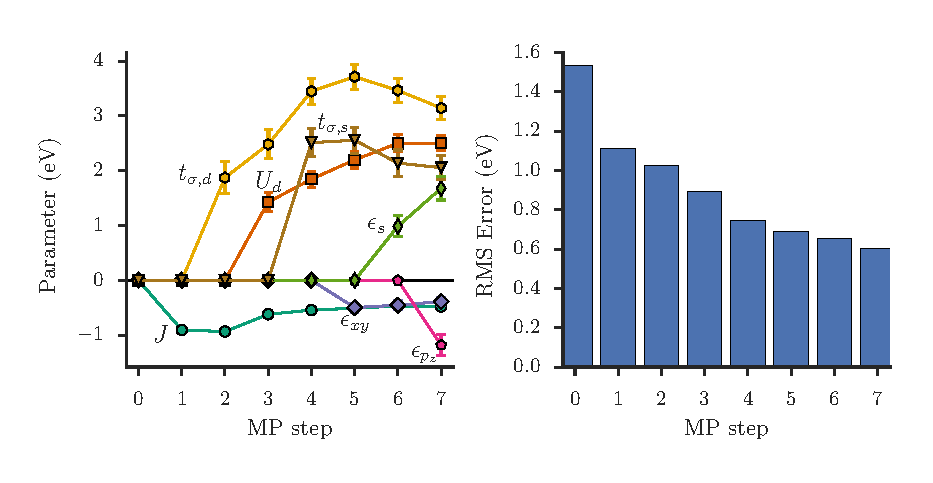
\includegraphics[width=0.8\textwidth]{./Figures/fese.eps}
  \caption{
    \label{fig:fese} 
    (Left) Parameter values for each fit generated in the MP algorithm, labeled at the step where they are included in the model. 
    A zero value indicates that parameter is not yet added to the model.
    The sign of $J$ is consistent with Hund's rules, and the signs of $t_{\sigma,d}$ and $t_{\sigma,s}$ are consistent with Se being located in positive $z$ with respect to Fe. 
    (Right) RMS error of each model generated by MP as the algorithm includes parameters. 
    The RMS error of the largest model considered was 0.61~eV.
  }
\end{figure*}


